\chapter{A review on player modeling for experience optimization}\label{ch:review_playing_optimization}
In virtual games, player modeling is best defined as the study of the use of artificial and computational intelligence techniques for the construction of models of players in dimensions regarding behavior, cognition, and affective states as well as beyond-game high level aspects spanning personality and cultural background~\citep{yannakakis_player_2013}. The idea behind such models is related to the goal of enabling a game to adjust the capability of its components and attributes towards an individual player satisfaction~\citep{herik_opponent_2005}. This idea has largely increased in importance over the last years. As one of the central reasons for that, is the increasing complexity of modern games fostered by the enhancement in computing power and graphics, as well as the commercial strategy of personalizing gaming experience~\citep{teng_customization_2010, herik_opponent_2005}. This chapter presents a brief overview of works targeting experience optimization, organized in three main parts, focusing on different aspects related to play experience optimization, namely: \textit{cognition}, \textit{behavior} and \textit{affection}. A relationship between our work and what proposed in literature is also presented.

\section{Focus on cognition and theoretical models of behavior}
One way researchers have addressed player modeling in games is by relying on theoretical frameworks mainly supported by psychology and neuroscience factors~\citep{yannakakis_player_2013}. By doing so, cognition aspects -- broadly seen as a set of all mental abilities and processes related to knowledge, such as: attention, memory, evaluation, reasoning, problem solving and decision making, learning and so forth -- are often investigated. 

Researches focused on theoretical framework of behavior are described in~\cite{yannakakis_player_2013} as being model-based. In this sense, they follow the \textit{modus operandi} of Humanities and Social Sciences which work, according to the authors, by coming up with a hypothetical model in advance, and investigate to what extent it fits the observations. When concerning the development of engaging experiences in entertainment systems,~\cite{yannakakis_how_2008} states that a comprehensive review of the literature regarding the elicitation of qualitative features and criteria derived from experimental psychological studies reveals a tendency of overlapping with the exploitation of theories of \textit{fun}, such as those discussed in~\cite{malone_what_1980},~\cite{lazzaro_why_2004} and~\cite{koster_theory_2013} envisioning to drive game design, as well as \textit{flow}~\citep{csikszentmihalyi_flow:_1991} (often used as a way of evaluating player enjoyment~\citep{sweetser_gameflow:_2005, cowley_toward_2008} (Fig.~\ref{flowDiagram})) and concepts like \textit{immersion}~\citep{calleja_digital_2007}. Most acceptably, according to theses theories and concepts, player engagement is most related to factors such as challenge, curiosity and fantasy.

\begin{figure}[htp]
  \centering  
  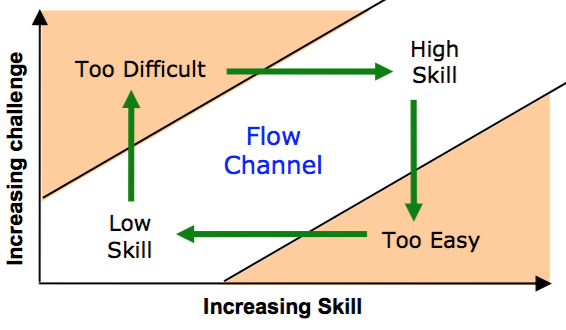
\includegraphics[draft=false]{images/02-art/flowDiagram.png}
  \caption{A flow diagram from~\cite{hunicke_ai_2004}. The figure shows the relationship between skill and level of challenge derived from the theory of flow~\citep{csikszentmihalyi_flow:_1991}. The point is to keep these two dimensions in a kind of positive correlation, meaning an increase that roughly approximates the diagonal.}
  \label{flowDiagram}
\end{figure}

Models aligned with cognition theories are seen as a valuable opportunity for understanding what the user is thinking when playing, which has direct relation with the ultimate desire of making the game respond intelligently to the player. According to~\cite{bohil_cognitive_2007}, the fundamental advantage of a direct focus on modeling principles supported by a theory of cognition is that it provides dynamic view at the individual player level, since it is possible to make statements about attention, learning, decision strategies, biases, an so on, unraveling indicators of the mental underpinning of observable behavior. 

The design of better~\gls{npc}s, for instance, is one of the central areas positively affected by the focus on cognition~\citep{funge_ai_1999}. Intuitively, once it is possible to measure some cognitive-related characteristics in the player (e.g., the attention level with respect to some in-game resource) it is possible to use them to steer the~\gls{npc} behavior towards the improvement of a desired~\gls{ai} capability -- Adaptive difficulty adjustment is one of these capabilities. Indeed, game difficulty is seen as having a direct link with challenge and fun, acting as source of satisfaction~\citep{koster_theory_2013,yannakakis_modeling_2006}. 

Cognitive models of players were also investigated with respect to psychological and cognitive neuroscience motivated question trough assessing physiological and/or psycho-physiological states during play. For instance, brain imaging techniques have been used to understand brain activity patterns related to aggressive thought stimulated via violent game content ~\citep{weber_does_2006}. The work of ~\cite{baumgartner_neural_2006} used Electroencephalography (EEG) combined with psychometric measures, as a first attempt to investigate neurophysiological underpinnings of spatial presence\footnote{spatial presence is considered as a sense of being physically situated within a spatial environment portrayed by a medium, such as television and virtual reality.} triggered in different virtual roller coaster scenarios.

Optimistically, as seen in~\cite{bohil_cognitive_2007}, the major point in cognition or related framework-based approaches for player modeling is to discover which model inputs -- in the sense of a parametric representation of cognition aspects -- place, for instance, unrealistic demands on a specific cognitive function, such as attention. Successful results on this, might heavily equip researches and game developers with valuable guidance for narrowing the range of necessary resource-consumption when aiming for desired results.   

\section{Focus on in-game actions, and behaviors}\label{sec:in_game_action_reviews}
A classical trend in player modeling is to investigate how primitive in-game activities can be used to describe the general behavior of the player. Originally, the first attempts for modeling players in this context used classical zero-sum board games (like chess, checker and go) as test-beds mainly by implementing search/heuristic methods to find the best moves in the game-tree. According to~\cite{bakkes_player_2012}, since tree-search techniques use evaluation functions in order to assess the pay-off of a particular move, they may be considered player models.

In-game actions are building blocks for any standard behavioral modeling approach. Most commonly, primitive actions are the unique way to identify player's preferences and decision-making style. Additionally, this modeling dimension is transferable across different game genres. A sequence of low-level actions -- such as moving from one direction to another -- is generally related to a classifiable behavior, such as ``attacking'', ``defending'', ``fleeing'', etc. In the RoboCup soccer league, for instance, a sequence of actions 9including targeted movements towards the opponent goalie may be commonly (and generally) classified as an ``attack''. Similarly, a sequence of actions intending to systematically prevent the opponent team from advancing on the field may be characterized as a ``defensive'' behavior. From this example, it is quite natural to realize that actions encode behaviors by perhaps acting as a kind of representation language for them. The important bit is that by keeping track of performed actions it is possible to find patterns that can be reasonably grouped together under the concept of a specific behavior. As discussed, actions were providing the raw information in most modeling approach for competitive advantage in section~\ref{compadvantage}.

Although classifying behaviors in this way may be relatively easy for simple, fully observable environments that involve a few possible deterministic actions and abstract behaviors, this classification process is limited in modern complex games since they normally have a large state-action space. Moreover, often behaviors lack the existence of a clear crossing point between them, and this makes the construction of player models even more challenging. Giving the size of the state-space, researchers have also to deal with the uncertainty involved in the fact that different action sequences may be related to the same behavior, while having a close relation with others. The fact that action sequence detection may be noisy is important, and also a challenge that has to be taken into account when using low-level actions to model behavior.  Furthermore, while computational constraints (such as memory demand) are the big key point, for instance, in search methods applied to turn based games, the dynamic characteristics in other types of games is the key. In~\gls{pirg}s, the inherent dynamism of the environment demands a special treatment of these aspects.

Besides all computational constraints involved and discussed in the previous paragraph, one might also see  the necessity of having different levels for behaviors. For instance, one might be interested on identifying when the player is mindless attacking, or when the player is using a full-fledged plan for performing the attack. In this context, what is the characteristic that separates these two behaviors? Again, using the RoboCup soccer league as an example,~\textit{is the player engaged in a proper ``attack'' or just keeping the ball in the attack field perhaps for the purpose of spending time?} Note that a ``proper'' attack may have more structured actions, perhaps including well-known patterns as opposed to a behavior of just ``spending time'', which in this case may use different sequences of actions.

The work of~\cite{bakkes_player_2012} presents an extensive discussion about the use of actions for player modeling, envisioning game experience optimization. In the authors' understanding, action models seem to be an attractive possibility for a model, since, once being able to predict accurately the future action that the player will take, acting accordingly would be a relatively easy task. However, they agree that the use of such models are limited unless when applied to relatively simple games. The justification for this is also related to the complexity of state-action space in state-of-art games. The authors also deem three more subdivisions for the topic, reported on Table~\ref{actionModels}.

\begin{table}[!ht]
\centering
\caption{The classification proposed by~\cite{bakkes_player_2012} for dimensions used in player modeling techniques based on virtual in-game actions.}
\label{actionModels}
\begin{tabularx}{\textwidth}{|c|X|} \hline
\textbf{Type of model}&\textbf{Brief description}\\ \hline
Tactic-based & relates to the automatic identification of short-term behavior as composed from actions targeting the achievement of a specific local goal. A common well-exploited concept is \textit{formation of game characters} which can be defined as a disposition of certain game agents.\\ \hline
Strategic-based & concerns global-term game behavior assessed via tactics sequences. This behavior may span over the entire game, some iterations of it or even across distinct genres of games.\\ \hline
Profiling-based & concerns psychological motivation for tactics and strategies.\\ \hline
\end{tabularx}
\end{table}

The divisions presented in Table~\ref{actionModels} are, in fact, not mutually exclusive and one can see them in a loose hierarchical manner. In other words, tactical-based models depend on action-based ones and, in the same way, strategy-based models may comprise a behavior inferred with the help of the previous two, etc. The main advantage, of modeling tactics over actions, however, is that the state-space complexity decreases as a result of higher information abstraction. But, since they are interrelated with each other aiming to achieve an overarching goal, modeling tactics alone, according to the authors, is not enough for effective player behavior modeling, since strategic play assumptions, as a high-level motivation for tactics, is commonly not incorporated, therefore, these models cannot generalize well over the underlying intentions behind observed tactics.

Additional to the use of actions in the modeling context discussed in section~\ref{compadvantage}, they are also the raw material exploited on designing games that can adjust difficulty automatically in order to keep the player's engagement at a high. Specifically, along-side procedural content generation -- the concept of generating game content on the fly --~\gls{dda} has taken a large piece of the virtual game community.

In essence, the idea is pretty simple: start by measuring the player's skill or level of challenge (difficulty) at a given moment and, based on this, steer the game behavior towards a state much likely to be compatible (in skills or challenge level) with that of the player. Following this recipe,~\cite{andrade_online_2004, andrade_extending_2005} aimed at investigating the usage of Q-learning and a challenge function in a 2D fighting game scenario. In their work the authors came up with a challenge function strictly based on the difference between the~\gls{npc} and player's health. From this, a game is assumed to be balanced if the function fluctuates around zero. By using a regular Q-learning they get to choose different best actions so to force the algorithm to choose the ones that most likely, according to the challenge function, matches the perceived player skill. 

~\cite{hunicke_ai_2004}, in turn, addressed~\gls{dda} by considering the notion of inventory analysis, that is, the processes of analyzing what resources are immediately available to the player w.r.t. the current challenge level of the game. During the game process, they observe certain player's characteristics, for example the level of damage the player takes, in order to generate an indication for the necessity of system intervention. When needed, their system would adjust supply and demand or resources so to control overall game difficulty. Ideally, the authors target the reduction of necessary intervention so to make it as seamless as possible. The system aims at keeping the player at the flow channel~\citep{csikszentmihalyi_flow:_1991} by encouraging certain events to take place or not. For example, the system basically tries to predict when the player is repeatedly putting himself on a state where current means can no longer achieve global or local goals.
When this happens, the system intervenes helping the player to progress.

Not surprising, the notion of having a ``challenger function'' that helps to guide adaptation is pretty much ubiquitous in the adapting game literature. Furthermore, any system relying on~\gls{dda} should also be concerned about the timing implication of such technique, i.e., the implications regarding the good moment to perform an attempt towards adjusting the game. For beginners, this is because a high frequency of adaptation is more likely to give the appearance of instability and so cause the game to be perceived as random. This instability is often referred to as the ``rubber-band'' effect as the IA appears to wobble around its skill level if the (human) player is too good and, conversely, overrun the player when he plays equivalent to the~\gls{ai}. Here though, appears clear the difficulty involving designing challenger functions. In the experiments done by~\cite{hunicke_ai_2004}, the authors noticed that a reactive approach, i.e. adjustment of onset elements, may run the risk of disrupting the player's sense of disbelief contributing to make the interpretation of the game harder and also make it ``schizophrenic''.%TODO the previous paragraph seems related to adaptation more than to player modeling. It is a further step possibly deserving a section per se, if you have collected enough info.
%EWERTON: But this section is dedicated to modeling for adaptation, i.e., to experience optimization.

In~\cite{hagelback_measuring_2009}, the authors went further on pooling people's opinion for the sake of knowing if playing an even game is more entertaining over being superior all the time. On their case study 60 people participated and they took the opportunity to conduct experiments using static and dynamic agents for their game test-bed. The dynamic agent type was able to react to in-game player behavior (for instance, to the player losing game resources). The obtained results suggested the dynamic agents were providing most entertainment to players during play while static ones presented themselves as too easy or too difficult. The authors' research provided good evidence for the implementation of~\gls{dda}-based systems.

\cite{spronck_-line_2004} propose one of the most popular examples of player modeling in virtual games. In their method, called ``dynamic scripting'' and defined as an unsupervised online learning technique for games, they maintain several rule-bases, one for each class of computer-controlled agents. Rules in the bases are manually designed using domain-specific knowledge and every time a new agent of a particular class is generated, the rules to compose the agent script are extracted from the corresponding rule-base. In this approach, the probability that a rule is selected for a script is proportional to the weight value that is associated with the rule. Also, the rule-base adapts by changing the rule weights to reflect the success or failure rate of the associated rules in scripts. %TODO Adaptation? EWERTON: in 

It did not take long until researchers realized that using a challenge function would pave the way for black-box optimization algorithm. Much of the literature covers the attempt of using evolutionary techniques as the main technique for~\gls{dda}. Among these works, it is worth notice that of~\cite{olesen_real-time_2008}, where the authors use evolutionary techniques to evolve agents so to balance an estimated challenge rating for the player skill. The take-away idea is that of making agents with a minimal difference in skill (w.r.t the player) to survive more and, on the other hand, lower the fitness of the ones whose difference is larger.%TODO Adaptation?

~\cite{demasi_-line_2003} focused on the use of~\gls{cea}s  proposing some methods and strategies for online evolution in an action (real-time) game. In this game, the~\gls{npc}s is evolved towards improving difficulty levels. The author presents four different methods: one that uses game specific information; one that merges offline-evolved data with online evolution; two others that focus on using online data only and using offline and online data together. Considerable drawbacks in the approach are the slow learning rate and the one-direction way of evolution, always toward the optimizing behavior. %TODO Adaptation? EWERTON: 

\cite{sejrsgaard-jacobsen_dynamic_2011} took a different approach by using~\gls{bt}, a kind of hierarchical finite state machine for controlling~\gls{npc}s, in order to dynamically adjust the difficulty in a 2D fighting game. They basically tested two different approaches. First, the traditional approach of defining predefined behaviors (encoded on~\gls{bt}s) and finding a way to switch between models (behavior) at run-time. For this, they developed an algorithm for selecting~\gls{bt}s based on perceived conditions. The second method, however, adjusts difficulty by changing~\gls{bt} properties themselves at run-time, such as the probability associated with children of selector nodes. This last method, was the one that obtained high capability in balancing the game. As claimed by the authors, their method served as a proof of concept for a small sized scenario (simple 2D fighting game) leaving the possibility for further investigation in larger game scenarios. Here, pops out an opportunity for testing on a~\gls{pirg} context, perhaps by following the current trend on applying such technique in robotics~\citep{scheper_behavior_2015, pereira_framework_2015, marzinotto_towards_2014}. %TODO Adaptation?

In summary, approaches addressing~\gls{dda} must, before the definition of the challenge function, identify important game characteristics affecting game difficulty, and challenge level. The overall philosophy is the adjustment of the game behavior to the perceived player's game skill, which should be made as seamless as possible. A good survey about adaptation-related challenges in games and simulations could be found in~\cite{lopes_adaptivity_2011}. The reader may refer to it in order to see a deeper treat on the identification and discussion of main challenges associated with the domain and also promising directions for research. %TODO Adaptation!

\section{Focus on affection aspects}\label{affectmodeling}
Also, some trend has emerged aiming on assessing the player's affective state (mainly emotion) as a mean of measuring the quality of interaction provided by the game. Here, the goal is related to the task of inferring internal traits of the player, such as personality and preference, during game-play~\citep{van_lankveld_psychologically_2009}. Methodologies that take this approach are more towards a research domain known as \textit{affective user modeling}, where the key point is that of assessing, heavily by using affection models, the inner state of the player regarding motivations for actions either based on action selection or through physiological data~\citep{van_lankveld_psychologically_2009}.

Being able to identify emotional profiles in this domain is useful given that they target a direct characterization of enjoyment level. For instance, after realizing that the player is compatible with an extroverted and highly responsible profile, the game~\gls{ai} may engage the user in rapid and repeated shifts of events, like from calm situation to a long and intense chain of events, or even a steep increase on motion abilities for~\gls{npc}s agents when proximity aspects, for instance, are important~\citep{bakkes_player_2012}.

Working on this,~\cite{tognetti_modeling_2010} proposed a framework to estimate player enjoyment preference from physiological signals in a car racing game. They collected 5 physiological signals from players, namely:~\gls{bvp},~\gls{ecg},~\gls{gsr}, Respiration (RESP) and Temperature (TEMP). From these basic signals, they were able to extract features such as: Heart rate (from ECG and~\gls{bvp}); magnitude and duration of~\gls{gsr}; expiration/inspiration time, apnea in/out time, respiration interval (all three from RESP); upper/lower envelope of~\gls{bvp}. Their data analysis, using Linear Discriminant Analysis, showed correlation between reported enjoyment and the described features, motivating further application on the use of biological signals without making any assumption on players' in-game activity.

Yannakakis and Hallam have published lots of papers on the matter of capturing and modeling affective state of entertainment, targeting children physiological state during physical game play. In~\cite{yannakakis_modeling_2006} and \cite{yannakakis_entertainment_2008}, children's heart rate, blood volume pulse and skin conductance were analyzed in the Playware prototype playground~\citep{lund_playware_2005}. Their findings suggested that a higher average and maximum heart rate, a steeper blood volume appear to correlate with higher levels of reported entertainment in children of 8-10 years-old. Essentially, the main effort is related to modeling entertainment based on selecting a minimal subset of individual features that are able to construct the quantitative user model for predicting the children's reported entertainment preferences. In doing so, they tested large margin algorithms (based on the~\gls{svm} principle) and Evolving Artificial Neural Networks. Successive works investigated feature selection and extend the approach for computer games~\citep{yannakakis_towards_2006,yannakakis_entertainment_2007,yannakakis_feature_2007,yannakakis_entertainment_2008-1}. 

There are indeed plenty of papers proposing the use of physiological data in game research. A widespread understanding is that measures from these methods are known for providing sensitive ways to assess the game experience, but they are hard to deal with since very often they require controlled experiments. In order to know more about this trend of research, the reader may refer to~\cite{kivikangas_review_2011} whose work presents a review focused on psycho-physiological methods for game research. For what concerns~\gls{pirg}s, physiological data are affected also by physical activity, thus behavior or emotion modeling based on these data could be negatively affected by the intrinsic way of playing this type of games.   
 
\section{Existing review papers and taxonomies}\label{reviews}
Taxonomies and reviews for player modeling have been recently proposed. \cite{smith_inclusive_2011} state that ``player modeling'' is a lose concept, since it can equally apply to everything from a predictive model of player actions resulting from machine learning to a designer's description of a player's expected reactions in response to some piece of game content. The authors introduced a broad taxonomy for the purpose of distinguishing between the major existing player modeling applications and techniques. Four facets were suggested: the scope of application, the purpose of use, the domain of modeled details, and the source of a model's derivation or motivation. The expectation involved is that the taxonomy would allow the identification of relevant player modeling methods for particular problems and clarify roles that a player model can take. As pointed out in the previous section, the work of~\cite{bakkes_player_2012} focuses on player behavioral modeling via in-game measurement of the human player distinguishing four types of player models: tactical models, strategic models, and player profiling. %TODO In the table 5.1, they were only 3, action models missing. Try to be consistent.
Through their examination, they noticed that these models are increasingly resource-intensive to build, but they also have an increasing tendency to generalize better.%TODO better than what?

\cite{machado_player_2011} also proposed and discussed a taxonomy for player modeling research gathering and organizing information from several different sources. They, in turn, tried to characterize the most important topics in the area expanding the discussion from~\cite{herik_opponent_2005} about the most common techniques, further presenting a new set of techniques. Additionally, they did an analysis of player modeling research possibilities in several game genres and also listed suitable game platforms for experimentation, discussing main characteristics.

Targeting a holistic view of player modeling with the aim of providing a high level taxonomy and discussion of key components of a player model,~\cite{yannakakis_player_2013} cluster the field into either \textit{model-based} approaches -- those that are built on a theoretical framework -- or \textit{model-free} ones -- those that refer to the construction of a model between player input and a player state representation by mainly relying on the \textit{modus operandi} of exact science, through computational techniques related to~\gls{ai} and~\gls{ml}. Additionally, they present a discussion about inputs and outputs to computational methods described as well as applications and current key challenges the field faces which are correlated to the inputs and outputs for the mentioned computational models.

\begin{table}[!ht]
\centering
\caption{Summary of existing popular survey-like papers concerning player modeling. {\mycirc} stands for proposal of taxonomy, {\mystar} stands for overview of literature and {\mydtriangle}, in turn, correspond to survey or review.}
\label{summaryReviews}
\begin{tabularx}{\textwidth}{|c|c|X|} \hline
\textbf{Paper}&\textbf{Type}&\textbf{Brief description}\\ \hline
\cite{smith_inclusive_2011}	& {\mycirc} & Build a broadly applicable taxonomy that can describe player modeling techniques across all games , both digital and non-digital, and in all games genres.\\ \hline
\cite{bakkes_player_2012} 	& {\mycirc} & An overview of methods by detailing four distinct approaches for modeling behaviour of players, namely: modeling player actions, modeling player tactics, modeling player strategies and player profiling. \\ \hline
\cite{yannakakis_player_2013} & {\mycirc},{\mystar} & A holistic view of player modeling, a high level taxonomy and discussion of key components as well as a description of challenges currently faced in the topic.\\ \hline
\cite{bakkes_personalised_2012} & {\mystar} & Motivation concerns for the topic, an broader overview, and  adaptive components for personalised games\\ \hline
\cite{machado_player_2011} &{\mydtriangle},{\mycirc} & Presents a survey of the field, discussing the main concepts and proposing a general taxonomy. \\ \hline
\cite{karpinskyj_video_2014} & {\mydtriangle} & Highlight most relevant trends and directions of research for the task of designing personalisation in games.\\ \hline
\end{tabularx}
\end{table}

Focusing on the point of personalized game experience in general,~\cite{bakkes_personalised_2012} provides a motivation for the promotion of methodologies in the topic as well as an extensive overview of scientific literature. To the former objective, they describe psychological foundations, the effect of satisfaction, the advantages to game development and requirements for achieving ambitions. To the extent of the overview, they go pretty much in the same direction of what has been exposed in~\cite{bakkes_player_2012}, however providing an intensive discussion about \textit{components of personalized games}, namely: space adaptation, mission/task adaptation, character adaptation, game mechanics adaptation, narrative adaptation, music/sound adaptation, player matching and difficulty scaling. An additional discussion about the relationship between personalized gaming and procedural content generation as well as the generalization to other domains (such as ambient games, human-computer interaction) is also mentioned.

Similarly, the work of~\cite{karpinskyj_video_2014} touches the subject of surveying the most relevant trends and directions of research in personalisation of computer games, to the extent that it is a true multi-disciplinary problem requiring contribution from areas as diverse as artificial and computational intelligence, game studies, psychology, game development and human computer interaction. Their survey considers five dimensions enabling to distinguish players from each other: preference, personality, experience, performance, and in-game behavior. Their discussion also aims to identify key research avenues that require further exploration. Table~\ref{summaryReviews} summarizes the most important points in the mentioned papers. 

Competitive advantage and/or experience optimization (section~\ref{ch:review_playing_optimization}) 
are not the unique types of approaches. There were also attempts for classifying opponent behavior to support the design of the game itself. An example of this is the work of~\cite{etheredge_generic_2013} where it is possible to see the implementation of fuzzy cluster analysis and~\gls{hmm} for finding player styles. %TODO Shouldn't this stay in player modeling section? Why is it here, in the "review papers" section?
The approach works as a classification method for player behavior, defined as a sequence of game actions. It consists of three components: interaction registry, cluster analysis and~\gls{hmm}. The first, serves as a data storage for actions maintaining a cumulative score value for them. The idea behind this is that actions that are not frequent are going to have an exponentially decreasing value in importance. On the other hand, frequently used actions have high importance score. These importance values for actions then constitute a primary source of information that is going to be used by cluster analysis as a way to group, i.e. classify, the player's styles.~\gls{hmm} is then used during game-play aiming to classify new players, as they play, and helping to spot appropriate and dependent game adjustments. The author claimed their method would be able to be used across different games (given their definition of player behavior) which can be considered as a possible generic design tool.

%TODO the same comment holds for the following one
Using the Rush 2008 American football simulator,~\cite{laviersa_using_2014} introduced methods for performing predictions about the players' physical movements when learning team policies. When focusing on recognition of team play they investigated the use of~\gls{svm}, an optimal margin classifier commonly used in supervised learning problems. They trained~\gls{svm}s for a multi-class objective by using a collection of simulated games under controlled conditions, so they got instances of every possible combination of offense and defense plays from a number of team starting formation configurations. The output of the play recognizer was defined as the system's best guess (at the current time step) about the opponent's choice of defensive play. Thus, they could use this information to select the most appropriate offense.

%TODO the same comment holds for the following one
Also in~\cite{laviersa_using_2014}, the authors focused on proposing methods for discovering how to effectively  subgroup agents together so to accomplish a given formation task, similar to~\cite{stone_task_1999}. Here again they based their method on an analysis of game data from successful team plays. The idea was to implement a supervised learning mechanism in order to identify important groups of players in each play. It is interesting to mention the three general types of cues that were used for the purpose of subgroup extraction: \textit{spatial} -- i.e, the constant relationships between team members over a period of time; \textit{temporal} -- co-occurrence of related actions; \textit{coordination} -- dependencies between members' actions. These cues turn out to be basics features for most types of approaches in the discussed scenario. Undoubtedly, a larger number of papers focused on player modeling for improving playing experience as to maximize the chances of maintaining the player engaged. 
%TODO To eliminate, I imagine -> This is the topic of discussion of the next section.

\section{Our work and the literature}
In accordance with what exposed so far, our research concentrated the aspects of playing for entertainment maximization aiming at developing new strategies for supporting acceptability of~\gls{pirg}s. To what concerns the literature, we define our work as related to the application of latent~\gls{ml}-model-based approaches %TODO Do I have missed this term in the classification? If you refer to the chapter just above, you should use the same classification terms.
to the problem of modeling the general behavior of a player. 

Our work concentrated on the exploitation of classification and clustering to differentiate among players. We have focused on modeling physical behavior and show how such aspect of interaction can be used to achieve player categorization and eventual robot adaptation. In terms of the related works presented above, we tend to be related to approaches that model the in-game activity as those presented in section~\ref{sec:in_game_action_reviews}. The main concerns in this phase are depicted in the conceptual relationship in the graph in figure~\ref{graph:ENGAGEMENT_structure}. %TODO It has to be clear to us, and to the reader, that ENGAGEMENT IS NOT ENTERTAINMENT. A part the problems in the correct and formal definition of the two terms, which should be provided, we cannot just assume that engaged people is also enjoying the game. For sure if engaged, he is motivated to play

\begin{figure}[ht]
    \centering
    \begin{tikzpicture}[ every annotation/.style = {draw,
                         fill = white, font = \Large}, scale=0.75,transform shape]
                         
      \path[mindmap,concept color=black!40,text=white,
        every node/.style={concept,circular drop shadow},
        root/.style    = {concept color=black!40,
          font=\large\bfseries,text width=10em},
        level 1 concept/.append style={font=\Large\bfseries,
          sibling angle=60,text width=7.7em,
        level distance=15em,inner sep=0pt},
        level 2 concept/.append style={font=\bfseries,level distance=9em},
      ]
        node[concept, font=\fontsize{16pt}{17pt}\selectfont\bfseries] {Engagement\\ Optimization}
        [clockwise from=0]
        child[concept color=green!50!black] {
          node[concept] {Player\\Modeling}
          [clockwise from=90]
          child { node[concept] {Behavior} }
          child { node[concept] {Learning} }
          child { node[concept, scale= 1.2, font=\fontsize{7pt}{17pt}\selectfont\bfseries] {Engagement} }
        }
        child[concept color=orange] { node[concept] {Difficult\\Selection}
        child { node[concept, scale=1.5, font=\fontsize{7pt}{17pt}\selectfont\bfseries] {Deception} }
        };
    \end{tikzpicture}
    \caption{Some relevant concepts in the engagement optimization dimension for our ~\gls{pirg} agent.}
    \label{graph:ENGAGEMENT_structure}
\end{figure}

Player modeling here takes into consideration several aspects like the general behavior (usual in-game actions), learning curve (changes in the usual behavior) and engagement (direct modeling of engaging variables). 

For all effects, we concentrated on tackling the general behavioral aspects so as to avoid the complexity of modeling dynamics. However, as one can see, the latent modeling algorithm we use can be easily extended to allow for modeling dynamics. This is in fact a direction of future work.

Additionally to modeling the player, we also investigated the advantages of implementing deceptive navigation and how this relates to self-reported game acceptability. The results indicate the need to further explore the concept and to isolate variables that can make the player perceiving the deceptive behavior. 